
\subsection*{Ejercicio 2.1}
En el problema de la braqu\'istocrona, se llega a que se debe minizar el funcional
\eq{
\label{integ}
 S=&\int_1^2 \sqrt{\frac{1+y'(x)^2}{ 2g y(x)}}dx\\
f=&\sqrt{\frac{1+y'(x)^2}{ 2g y(x)}}.
}
La ecuaci\'on de Euler-Lagrange para el problema se obtiene facilmente haciendo los siguientes c\'alculos:
\eq{
\frac{\partial f}{\partial y'(x)}=&\frac{y'(x)}{\sqrt{(2 g y(x))(1+y'(x)^2)}}\\
\frac{\partial f}{\partial y(x)}=&\frac{\sqrt{1+y'(x)^2}}{2 y \sqrt{2 g y}}\\
0=&\frac{d\left(\frac{\partial f}{\partial y'(x)} \right)}{dx}-\frac{\partial f}{\partial y(x)}=\frac{d\left( \frac{y'(x)}{\sqrt{(2 g y(x))(1+y'(x)^2)}}\right)}{dx}-\frac{\sqrt{1+y'(x)^2}}{2 y \sqrt{2 g y}}\nonumber \\
=&-\frac{y'(x)^2+2 y(x) y''(x)+1}{2 \sqrt{2} g^2 y(x)^3
   \left(\frac{y'(x)^2+1}{g y(x)}\right)^{3/2}} .
}
La ecuaci\'on diferencial que debemos resolver es entonces:
\eq{
y'(x)^2+2 y(x) y''(x)+1=0.
\label{n}
}
Podemos notar que $f$ no depende explictamente de $x$, entonces la cantidad $h=\frac{\partial f}{\partial y'(x)}y'(x)-f$ es una cantidad conservada. Para este caso $h$ tiene la siguiente forma:
\eq{
h=&-\frac{1}{\sqrt{2 g y(x)(1+y'(x)^2)}}=\text{cte} \\
\frac{1}{h^2}=&2 g y(x) (1+y'(x))^2.
}
Si se deriva la \'ultima de las ecuaciones con respecto a $x$ se llega a :
\eq{
0= \frac{d \left(\frac{1}{h^2}\right)}{dx}=g y'(x) \left(y'(x)^2+1\right)+2 g y(x) y'(x) y''(x)
}
Que es la misma ecuaci\'on (\ref{n}) multiplicada por $g y'(x)$. Es decir la ecuaci\'on (\ref{n}) es equivalente a $y(x) (1+y'(x)^2)=2c$. De esta ecuaci\'on se puede despejar $y'(x)$ separar variables e integrar para obtener :
\eq{
 y'(x)^2=&\frac{2c}{y}-1\\
\frac{dy}{\sqrt{\frac{2c}{y}-1}}=&dx\\
 2 c \tan ^{-1}\left(\frac{1}{\sqrt{\frac{2
   c}{y}-1}}\right)-\sqrt{(2 c-y) y}  =&x.
}
Pero $\tan^{-1}(x)=\cos^{-1}\left(\frac{1}{\sqrt{1+x^2}}\right)$ entonces:
\eq{
2 c \cos ^{-1}\left(\sqrt{1-\frac{y}{2
   c}}\right)-\sqrt{(2 c-y) y}=x\\
1-\frac{y}{2c}=\cos^2\left(\frac{x+\sqrt{y(2c-y)}}{2c}\right).
}
Llamando $\alpha=\frac{x+\sqrt{y(2c-y)}}{c}$ y despejando:
\eq{
\frac{y}{2c}=1-\cos^2\left(\frac{\alpha}{2}\right)=\frac{1-\cos(\alpha)}{2}\\
\frac{y}{c}=1-\cos\left(\frac{x+\sqrt{y(2c-y)}}{c} \right)
}
La \'ultima igualdad se obtiene de las identidades de \'angulo mitad para el coseno.
De esta igualdad tambien se ve que $y$ s\'olo puede tomar valores en el intervalo $[0,2a]$ (ya que la que la cantidad dentro del radical del coseno s\'olo es mayor que 0 en este intervalo) y que uno de sus m\'inimos est\'a en $(0,0)$(que fue de donde se lanz\'o la part\'icula), es decir all\'i hay una c\'uspide.\\
Por otro lado para mostrar que si la part\'icula se proyecta con una energia cin\'etica inicial $\frac{1}{2}m v_0^2$ entonces tambien est\'a se mueve sobre un cicloide basta notar que la integral (\ref{integ}) se reescribe de esta forma (Conservaci\'on de Energia: $\frac{1}{2}m v_0^2=\frac{1}{2} mv^2-mgy$):
\eq{
S=\int_1^2 \sqrt{\frac{1+y'(x)^2}{2 g y(x)+v_0^2}}dx
}
Esta puede ser devuelta a su forma original haciendo el cambio de variable $\hat y=y+\frac{v_0^2}{2g}$, esto equivale a mover el sistema de coordenadas $\frac{v_0^2}{2g}$ unidades, por lo tanto la c\'uspide que estaba en $y=0$ quedar\'a $\frac{v_0^2}{2g}$ unidades mas arriba.


\subsection*{Ejercicio 2.3 }
La soluci\'on a este problema consiste en minimizar el funcional 
\eq{
J=\int_1^2 \sqrt{dx^2+dy_1^2+dy_2^2}=\int_{x_1}^{x_2} \sqrt{1+\left(\frac{dy_1}{dx}\right)^2+\left(\frac{dy_2}{dx}\right)^2}dx,
} para esto resolvemos:
\eq{
\label{eu}
0&=\frac{\partial f}{\partial y_i}-\frac{d}{dx} \left(\frac{\partial f}{\partial \dot y_i}\right)\\
f&=\sqrt{1+\dot y_1^2+\dot y_2^2}\\
\dot y_i&=\frac{dy_i}{dx},
}
con $f$ as\'i definida obtenemos:
\eq{
 \frac{\partial f}{\partial y_i}&=0\\
\frac{\partial f}{\partial \dot y_i}&=\frac{\dot y_1}{\sqrt{1+\sum_i\dot y_i^2}}.\\
}
as\'i llegamos a que:
\eq{
\frac{d}{dx}\left(\frac{\dot y_i}{\sqrt{1+\sum_i\dot y_i^2}}\right)=0\\
\frac{\dot y_i}{\sqrt{1+\sum_i\dot y_i^2}}=c_i.
}
La \'ultima ecuaci\'on se puede solucionar para las $y_i$:
\eq{
\dot y_i^2= \frac{c_i^2}{1-\sum_i c_i}
}
y finalmente:
\eq{
y_i=a_i x +b_i
}
Las anteriores son las ecuaciones de una recta parametrizadas por la primera de sus coordenadas.

\subsection*{Ejercicio 2.4 }
Con un procedimiento an\'alogo al anterior pero usando coordenadas esf\'ericas $(r,\theta,\phi)$ (con $r$ fijo) llegamos a que $ds^2=r^2(d\theta^2+\sin^2 \theta d\phi^2) $ llegamos al siguiente funcional
\eq{
 F=\int_1^2 \sqrt{d\theta^2+\sin^2\theta d\phi^2}=\int_{\theta_1}^{\theta_2}{\sqrt{1+\sin^2\theta \left(\frac{d\phi}{d\theta}\right)^2} d\theta}.
}
Haciendo uso de (\ref{eu}) pero con $f=\sqrt{1+\sin^2\theta \left(\frac{d\phi}{d\theta}\right)^2}$ , $y_i=\phi$ , $x=\theta$ y $\dot \phi=\frac{d\phi}{d\theta}$
obtenemos lo siguiente:
\eq{
\frac{\partial f}{\partial \phi}&=0\\
\frac{\partial f}{\partial \dot \phi}&=\frac{\sin^2 \theta \dot \phi}{\sqrt{1+\sin^2 \theta  \dot \phi^2}}\\
0&=\frac{d }{d\theta} \left(\frac{\sin^2 \theta \dot \phi}{\sqrt{1+\sin^2 \theta  \dot \phi^2}}\right).
}
De la \'ultima ecuaci\'on deducimos que:
\eq{
\frac{\sin^2 \theta \dot \phi}{\sqrt{1+\sin^2 \theta \dot \phi^2}}=C_1.
}
De esta y la anterior podemos despejar $\dot \phi$ e integrar para obtener:
\eq{
\dot \phi&=\pm \frac{C_1 \csc (\theta )}{\sqrt{\sin ^2(\theta )-C_1^2}}\\
\label{pi}
\phi(\theta)&=C_2 \pm \tan ^{-1}\left(\frac{\sqrt{2} C_1 \cos (\theta
   )}{\sqrt{-2 C_1^2-\cos (2 \theta )+1}}\right)=C_2 \pm \tan ^{-1}\left(\frac{ \cos \theta
   }{\sqrt{\frac{\sin^2 \theta }{C_1^2} -1}}\right).
}
Ahora nos falta mostrar que la anterior ecuaci\'on define un c\'irculo m\'aximo. Para esto es suficiente con mostrar que el plano en el que esta la curva que hemos encontrado anteriormente pasa por el origen.
Para lo anterior note que $\tan^{-1}(x)=\sin^{-1}\left(\frac{x}{\sqrt{1+x^2}}\right)$ y por lo tanto la ecuaci\'on (\ref{pi}) se  puede reescribir as\'i :
\eq{
\phi-C_2=\tan^{-1}\left(\frac{\cot \theta}{\sqrt{\frac{1}{C_1^2}-\csc^2\theta}   }  \right)=\sin^{-1} \left(   \frac{\frac{\cot \theta}{\sqrt{1/C_1^2-\csc^2 \theta}}}{\sqrt{1+\frac{\cot^2\theta}{1/C_1^2-\csc^2\theta}}} \right)\\
\sin^{-1}\left(\frac{\cot \theta}{\sqrt{1/C_1^2+\cot^2 \theta -\csc^2 \theta}}\right)=\sin^{-1}\left(\frac{\cot \theta}{\sqrt{1/C_1^2-1}} \right)
}
o:
\eq{
 \sin{\phi-C_2}&=\left(\frac{\cot \theta}{\sqrt{1/C_1^2-1}} \right)\\
\sin \phi \cos C_2-\sin C_2 \cos \phi &=\left(\frac{\cot \theta}{\sqrt{1/C_1^2-1}} \right)\\
\sin \theta \sin \phi \cos C_2-\sin \theta \sin C_2 \cos \phi&=\frac{\cos \theta}{\sqrt{1/C_1^2-1}}.
}
Pero $x=r \cos \phi \sin \theta$, $y=r \sin \phi \sin \theta$, $z=r \cos \theta$ y la \'ultima ecuacion queda:
\eq{
y \cos C_2-x\sin C_2=\frac{z}{\sqrt{1/C_1^2-1}}
}
que define un plano que pasa por (0,0,0). Note que en la ecuacion anterior $x,y$ y $z$ son funciones de $\theta$ por lo que describen una curva y no un plano.

\subsection*{Ejercicio 2.6}
Del problema que estamos considerando se nota facilmente que la fuerza que atrae a la part\'icula es proporcional a la distancia y est\'a en la direcci\'on radial, por lo tanto el potencial asociado a dicha fuerza es de la forma $V(r)=\frac{1}{2} k r^2$. Escogeremos nuestro sistema de referencia con el origen en el centro de la esfera y con el eje $z$ perpendicular al plano donde se hara el tunel. Asi entonces llegamos a que la energia de la part\'icula que estamos considerando viene dada por:
\eq{
E=\frac{1}{2}m (\dot r^2+r^2 \dot \theta^2)+\frac{1}{2} k r^2=\frac{1}{2}k a^2
}
Donde $a$ es el radio de la esfera en la que se mover\'a la part\'icula, $\dot w$ denota derivada total con respecto a $t$ mientras $w'$ denota derivada con respecto $\theta$ y $k=\frac{G M m}{a^3}$. De la anterior ecuaci\'on se puede despejar facilmente ``$dt$'' para obtener:
\eq{
\int dt=\int f d\theta=\sqrt{\frac{m}{k}}\int \sqrt{\frac{r(\theta )^2+r'(\theta )^2}{a^2 - r(\theta
   )^2}} d \theta
}
Al escribir las ecuaciones de Euler-Lagrange para minimizar $\int dt$ se obtiene:
\eq{
\frac{r(\theta ) \sqrt{\frac{m \left(r(\theta
   )^2+r'(\theta )^2\right)}{k \left(a^2-r(\theta
   )^2\right)}} \left(r''(\theta ) r(\theta
   )^3+\left(a^2-r'(\theta )^2\right) r(\theta )^2-a^2
   r''(\theta ) r(\theta )+2 a^2 r'(\theta
   )^2\right)}{r(\theta )^2+r'(\theta )^2}=0
}
De la anterior igualdad la ecuaci\'on relevante es:
\eq{
r''(\theta ) r(\theta )^3+\left(a^2-r'(\theta )^2\right)
   r(\theta )^2-a^2 r''(\theta ) r(\theta )+2 a^2
   r'(\theta )^2=0
}
Aunque la anterior ecuaci\'on se ve algo complicada esta se puede integrar una vez al notar que $f$ no depende de $\theta$ y por lo tanto:
\eq{
\sqrt{I}=\frac{\partial f}{\partial r'(\theta)} r'(\theta)-f=\frac{r(\theta )^2 \sqrt{\frac{m \left(r(\theta
   )^2+r'(\theta )^2\right)}{k \left(a^2-r(\theta
   )^2\right)}}}{r(\theta )^2+r'(\theta )^2}
}
Es una cantidad conservada. La \'ultima igualdad se puede escribir de manera mas conveniente como:
\eq{
\frac{a^2 r^2}{a^2-r^2}\left(\frac{r^2}{I a^2}-1+\frac{r^2}{a^2}  \right)=r'(\theta)^2
}
Si redefinimos a $\frac{1}{I}=\left(-1+\frac{a^2}{r_0^2} \right)$ entonces la ecuaci\'on anterior queda asi:
\eq{
\frac{a^2 r^2}{a^2-r^2}\frac{r^2-r_0^2}{r_0^2}=r'(\theta)^2
}
Note que la ecuaci\'on anterior restringe los posibles valores $r$ a $r_0\leq r \leq a$ ya que la derivada de $r$ debe ser real.
De la anterior ecuaci\'on basta mostrar que es satisfecha por una hipocicloide


\begin{figure}
\centering
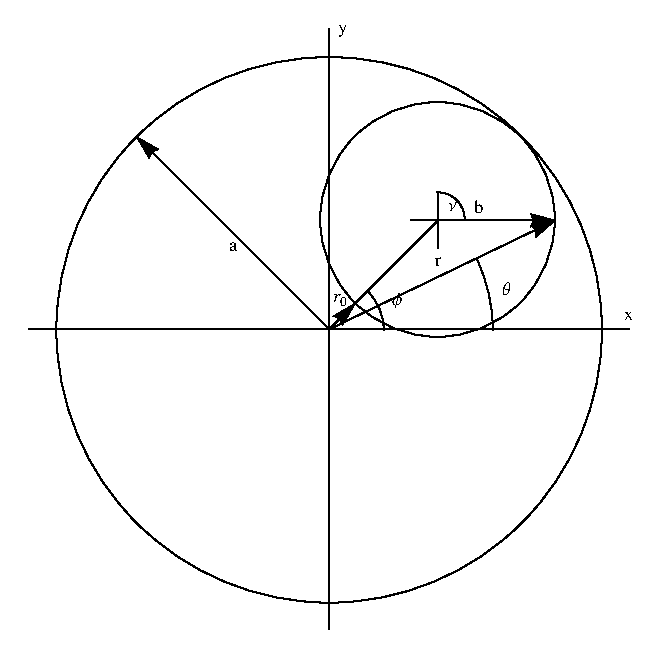
\includegraphics[width=0.9 \textwidth]{dib.eps}
\caption{Contrucci\'on de una hipocicloide: Sea $a$ el radio del circulo mayor y $b$ el radio del circulo menor. Sea $\theta$ el \'angulo que forma el vector de posici\'on del punto sobre el circulo menor con el eje $x$, sea $\phi$ el \'angulo que forma el centro del circulo menor y el eje $x$, finalmente sea $\nu$ el \'angulo que rota el circulo menor sobre un eje fijo. De la condici\'on de no deslizamiento se obtiene que $\nu=\frac{a-b}{b} \phi$. Podemos escribir la posici\'on del punto en t\'erminos de $\phi$ y $\nu$ asi (definimos a $r_0=a-2b$, la distancia mas cercana al centro):
$x=(a-b)\cos \phi-b \cos \nu=\frac{1}{2}\left((a+r_0) \cos (\phi)+(r_0-a) \cos \left(\frac{(a+r_0) \phi}{a-r_0}\right)\right)$
$y=(a-b)\sin \phi+b \sin \nu=\frac{1}{2}\left((a+r_0) \sin (\phi)+(a-r_0) \sin \left(\frac{(a+r_0) \phi}{a-r_0} \right)\right)$}
\label{a}
\end{figure}


Las ecuaciones par\'ametricas de una hipocicloide son:
\eq{
x(\phi)&=\frac{1}{2}\left((a+r_{0}) \cos (\phi)+(r_{0}-a) \cos \left(\frac{(a+r_{0}) \phi}{a-r_{0}}\right)\right) \\
y(\phi)&=\frac{1}{2}\left((a+r_{0}) \sin (\phi)+(a-r_{0}) \sin \left(\frac{(a+r_{0}) \phi}{a-r_{0}}\right)\right) 
}
De estas se puede obtener $r(\phi)^2$ asi:
\eq{
r(\phi)^2=x(\phi)^2+y(\phi)^2=&\frac{1}{4} \left((a+r_0) \cos (\phi
   )+(r_{0}-a) \cos \left(\frac{(a+r_{0}) \phi
   }{a-r_{0}}\right)\right)^2\\
&+\frac{1}{4}
   \left((a+r_{0}) \sin (\phi )+(a-r_{0}) \sin
   \left(\frac{(a+r_{0}) \phi
   }{a-r_{0}}\right)\right)^2 \nonumber
}
Que al simplificar teniendo en cuenta que $\cos^2 x+\sin^2 x=1$, $\cos(a+b)=\cos a \cos b-\sin a \sin b$ y que $(a+b)^2+(a-b)^2=2(a^2+b^2)$ queda:
\eq{
r(\phi)^2=\frac{1}{2}
   \left(a^2+r_{0}^2+\left(r_{0}^2-a^2\right)
   \cos \left(\frac{2 a \phi
   }{a-r_{0}}\right)\right)
}
Por otro lado tambien podemos calcular $\theta(\phi)$:
\eq{
\tan(\theta(\phi))=&\frac{y(\phi)}{x(\phi)}=\frac{(a+r_{0}) \sin (\phi )+(a-r_{0}) \sin
   \left(\frac{(a+r_{0}) \phi
   }{a-r_{0}}\right)}{(a+r_{0}) \cos (\phi
   )+(r_{0}-a) \cos \left(\frac{(a+r_{0}) \phi
   }{a-r_{0}}\right)}\\
=&\frac{a \sin (\phi )+r_{0} \sin (\phi )+a \sin
   \left(\frac{(a+r_{0}) \phi
   }{a-r_{0}}\right)-r_{0} \sin
   \left(\frac{(a+r_{0}) \phi
   }{a-r_{0}}\right)}{a \cos (\phi )+r_{0} \cos
   (\phi )-a \cos \left(\frac{(a+r_{0}) \phi
   }{a-r_{0}}\right)+r_{0} \cos
   \left(\frac{(a+r_{0}) \phi }{a-r_{0}}\right)}\\
=&\frac{r_{0} \left(\sin (\phi )-\sin
   \left(\frac{(a+r_{0}) \phi
   }{a-r_{0}}\right)\right)+a \left(\sin (\phi
   )+\sin \left(\frac{(a+r_{0}) \phi
   }{a-r_{0}}\right)\right)}{a \left(\cos (\phi
   )-\cos \left(\frac{(a+r_{0}) \phi
   }{a-r_{0}}\right)\right)+r_{0} \left(\cos
   (\phi )+\cos \left(\frac{(a+r_{0}) \phi
   }{a-r_{0}}\right)\right)}
}
Pero recordando las identidades de suma a producto de funciones trigonometricas se puede reescribir
\eq{
=&\frac{2 r_{0} \cos \left(\frac{(a+r_{0}) \phi
   }{2 (a-r_{0})}+\frac{\phi }{2}\right) \sin
   \left(\frac{\phi }{2}-\frac{(a+r_{0}) \phi }{2
   (a-r_{0})}\right)+2 a \cos \left(\frac{\phi
   }{2}-\frac{(a+r_{0}) \phi }{2
   (a-r_{0})}\right) \sin \left(\frac{(a+r_{0})
   \phi }{2 (a-r_{0})}+\frac{\phi }{2}\right)}{2
   r_{0} \cos \left(\frac{\phi
   }{2}-\frac{(a+r_{0}) \phi }{2
   (a-r_{0})}\right) \cos \left(\frac{(a+r_{0})
   \phi }{2 (a-r_{0})}+\frac{\phi }{2}\right)-2 a
   \sin \left(\frac{\phi }{2}-\frac{(a+r_{0}) \phi
   }{2 (a-r_{0})}\right) \sin
   \left(\frac{(a+r_{0}) \phi }{2
   (a-r_{0})}+\frac{\phi }{2}\right)}\\
=&\frac{a \cos \left(\frac{r_{0} \phi
   }{a-r_{0}}\right) \sin \left(\frac{a \phi
   }{a-r_{0}}\right)-r_{0} \cos \left(\frac{a
   \phi }{a-r_{0}}\right) \sin \left(\frac{r_{0}
   \phi }{a-r_{0}}\right)}{r_{0} \cos
   \left(\frac{a \phi }{a-r_{0}}\right) \cos
   \left(\frac{r_{0} \phi }{a-r_{0}}\right)+a
   \sin \left(\frac{a \phi }{a-r_{0}}\right) \sin
   \left(\frac{r_{0} \phi }{a-r_{0}}\right)}
}
si la anterior ecuaci\'on se divide en el numerador y en el denominador por $\cos \left(\frac{a \phi }{a-r_{0}}\right) \cos \left(\frac{r_{0} \phi }{a-r_{0}}\right)$ obtenemos:
\eq{\tan \theta(\phi)=\frac{a \tan \left ( \frac{a \phi}{a-r_0}\right)-r_0\tan \left ( \frac{r_0 \phi}{a-r_0}\right)}{r_0+a \tan \left ( \frac{a \phi}{a-r_0}\right) \tan \left ( \frac{r_0\phi}{a-r_0}\right)}
}
Note que la \'ultima ecuaci\'on tiene un notable parecido con la identidad suma de la tangente.\\
Con lo anterior calculado es directo calcular la siguiente cantidad:
\eq{
\tan\left(\theta + \frac{r_0 \phi}{a-r_0}  \right)=&\frac{\tan\left( \theta \right)+\tan\left( \frac{r_0 \phi}{a-r_0} \right)}{1-\tan\left( \frac{r_0 \phi}{a-r_0} \right)\tan\left(\theta  \right)}\\
=&\frac{\frac{a \tan\left( \frac{a \phi}{a-r_0}  \right)-r_0\tan\left( \frac{r_0 \phi}{a-r_0}  \right)+r_0\tan\left( \frac{r_0 \phi}{a-r_0} \right)+a \tan\left( \frac{r_0 \phi}{a-r_0} \right)\tan\left( \frac{a \phi}{a-r_0}  \right)\tan\left( \frac{r_0 \phi}{a-r_0} \right)}{r_0+a \tan \left ( \frac{a \phi}{a-r_0}\right) \tan \left ( \frac{r_0\phi}{a-r_0}\right)}}{\frac{r_0+a \tan\left( \frac{a \phi}{a-r_0} \right) \tan\left( \frac{r_0 \phi}{a-r_0} \right)-\left(a \tan\left( \frac{a \phi}{a-r_0} \right)    -r_0 \tan\left( \frac{r_0 \phi}{a-r_0} \right)\right) \tan\left( \frac{r_0 \phi}{a-r_0} \right)}{r_0+a \tan \left ( \frac{a \phi}{a-r_0}\right) \tan \left ( \frac{r_0\phi}{a-r_0}\right)}}
\\
=&\frac{a \tan\left( \frac{a \phi}{a-r_0} \right) \left( 1- \tan^2\left( \frac{r_0 \phi}{a-r_0} \right)\right)}{r_0 \left( 1- \tan^2\left( \frac{r_0 \phi}{a-r_0} \right) \right)}
}
Finalmente 
\eq{
\tan\left(\theta + \frac{r_0 \phi}{a-r_0}  \right)=\frac{a \tan\left( \frac{a \phi}{a-r_0} \right)}{r_0}
}
asi $\theta(\phi)$ es:
\eq{
 \theta(\phi)=\tan^{-1}\left(\frac{a}{r_0} \tan\left(\frac{a \phi}{a-r_0} \right) \right)-\frac{r_0 \phi}{a-r_0}
}

Ahora que conocemos $r(\phi)$ y $\theta(\phi)$ podemos calcular $r'(\theta)^2$ asi:
\eq{
\left(\frac{dr}{d\theta}\right)^2=\left(\frac{\frac{dr}{d\phi}}{\frac{d\theta}{d\phi}}\right)^2&=
\left(\frac{-\frac{a \left(r_0^2-a^2\right) \sin \left(\frac{2 a \phi }{a-r_0}\right)}{\sqrt{2}
   (a-r_0) \sqrt{a^2+r_0^2+\left(r_0^2-a^2\right) \cos \left(\frac{2 a \phi
   }{a-r_0}\right)}}}{\frac{a^2 \sec ^2\left(\frac{a \phi }{a-r_0}\right)}{(a-r_0) r_0
   \left(\frac{a^2 \tan ^2\left(\frac{a \phi
   }{a-r_0}\right)}{r_0^2}+1\right)}-\frac{r_0}{a-r_0}}\right)^2\\
&=-\frac{a^2 \left(-a^2-r_0^2+\left(a^2-r_0^2\right) \cos \left(\frac{2 a \phi
   }{a-r_0}\right)\right) \tan ^2\left(\frac{a \phi }{a-r_0}\right)}{2 r_0^2}
}
Por otro lado si calculamos el lado izquierdo de la ecuaci\'on diferencial 
\eq{
&\frac{a^2 r^2}{a^2-r^2}\frac{r^2-r_0^2}{r_0^2}\\
&\quad =\frac{a^2 \left(a^2+r_0^2+\left(r_0^2-a^2\right) \cos \left(\frac{2 a \phi
   }{a-r_0}\right)\right) \left(\frac{1}{2}
   \left(a^2+r_0^2+\left(r_0^2-a^2\right) \cos \left(\frac{2 a \phi
   }{a-r_0}\right)\right)-r_0^2\right)}{2 r_0^2 \left(a^2+\frac{1}{2}
   \left(-a^2-r_0^2-\left(r_0^2-a^2\right) \cos \left(\frac{2 a \phi
   }{a-r_0}\right)\right)\right)}
}
Que al simplificar se convierte en:
\eq{-\frac{a^2 \left(-a^2-r_{0}^2+(a-r_{0})
   (a+r_{0}) \cos \left(\frac{2 a \phi
   }{a-r_{0}}\right)\right) \tan ^2\left(\frac{a
   \phi }{a-r_{0}}\right)}{2 r_{0}^2}
}
Lo que muestra que efectivamente la hipocicloide es la solucion del problema.
\\
Por \'ultimo queremos calcular el tiempo de viaje y la profundidad m\'axima alcanzada en funci\'on de la separaci\'on angular de los puntos sobre la tierra.
Para encontrar las anteriores cantidades primero notemos $r_0\leq r\leq a$ y que $r_0=r \rightarrow \phi=0 \rightarrow \theta=0$, es decir por la forma como construimos la soluci\'on $r$ es m\'inimo en $\theta=0$. Ahora podemos buscar $\theta$ tal que $r=a$, para ello primero encontremos  a $\phi$ que cumpla esa condici\'on:
\eq{
a^2=\frac{1}{2}
   \left(a^2+r_{0}^2+\left(r_{0}^2-a^2\right)
   \cos \left(\frac{2 a \phi
   }{a-r_{0}}\right)\right) \rightarrow \phi=\frac{\pi}{2} \frac{a-r_0}{a}
}
Si reemplazamos lo anterior en la ecuaci\'on para $\theta$ se obtiene que:
$$\theta(r=a)=\frac{\pi}{2}\left(1-\frac{r_0}{a}\right)$$
Asi entonces el anterior es el \'angulo se barre entre ir de la superficie al punto de maximo acercamiento, por razones de simetr\'ia este debe ser igual al \'angulo que se barre en ir desde el punto de m\'aximo acercamiento al centro hasta la superficie de nuevo. De lo anterior se deduce entonces que si en el trayecto de viaje de el vehiculo se acerca hasta el centro $r_0$ entonces los puntos estan separados angularmente una distancia $\alpha=\pi \left(1-\frac{r_0}{a}\right)$. Como es de esperarse si los dos puntos son diametramente opuestos entonces $r_0=0$ y la trayectoria pasa por el centro y ademas como se comprueba facilmente es una linea recta en la que se presenta movimiento arm\'onico simple.\\
Finalmente la integral que da el tiempo de viaje se puede reparametrizar en terminos de $\phi$ para obtener:
\eq{
t_{min}&=\sqrt{\frac{m}{k}}\int_{-\frac{\pi}{2}(1-\frac{r_0}{a})}^{\frac{\pi}{2}(1-\frac{r_0}{a})} 
\sqrt{\frac{\left(\frac{dr}{d\phi} \right)^2+r^2(\phi)\left(\frac{d\theta}{d\phi} \right)^2}{a^2-r^2(\phi)}} d\phi\\
&=\sqrt{\frac{m}{k}} \frac{\pi}{a}\sqrt{a^2-r_0^2}=\sqrt{\frac{m}{k}} \pi\sqrt{1-\left(\frac{r_0}{a}\right)^2}
}
Pero $\frac{r_0}{a}=1-\frac{\alpha}{\pi}$ as\'i que el tiempo m\'inimo en t\'erminos de la separaci\'on angular es:
$$
t_{min}=\sqrt{\frac{m}{k}} \pi \sqrt{1-\left(1-\frac{\alpha}{\pi}\right)^2}
$$
Finalmente se pide hallar el tiempo de viaje entre Los \'Angeles y Nueva York. Estas ciudades estan separadas por una distancia de $4800$ km.AAdemas se sabe que el diametro de la Tierra es de aproximadamente $a=6400$ km luego su separaci\'on angular es de $\alpha=\frac{4800}{6400}=0.75$ ademas la masa de la Tierra es de $M=6.0\cdot10^{24}$ kg y la constante de Cavendish tiene un valor de $G=6.7 \cdot 10^{-11}$ m$^3$ kg$^{-1}$ s$^{-2}$ entonces $\frac{k}{m}=1.5 \cdot 10^{-6}$ s$^{-2}$.\\
El tiempo de viaje de Nueva York a Los \'Angeles es $t_{NY-LA}=1.64\cdot10^3$ s$=27'$ y el radio m\'inimo es $r_0=a \left(1-\frac{0.75}{\pi}\right)=4.9\cdot 10^3$ km.









\subsection*{Ejercicio 2.16}
Para el presente problema el Lagrangiano est\'a dado por :
\eq{
L=e^{t \gamma } \left(\frac{1}{2} m
   \dot q(t)^2-\frac{1}{2} k q(t)^2\right)
\label{kl}
}
La ecuaci\'on de Euler Lagrange para el anterior Lagrangiano es:
\eq{
e^{t \gamma } \left(k q(t)+m \left(\gamma 
   \dot q(t)+\ddot q(t)\right)\right)=0
}
Que es la ecuaci\'on de movimiento de un oscilador arm\'onico amortiguado.
Si se hace la transformaci\'on de coordenadas $q=e^{-\frac{t \gamma }{2}} s $ el Lagrangiano toma la forma siguiente:
\eq{
L'=\frac{1}{8} \left(\left(m \gamma ^2-4 k\right)
   s(t)^2-4 m \gamma  \dot s(t) s(t)+4 m
   \dot s(t)^2\right)
}
La ecuaci\'on de Euler lagrange es:
\eq{
\left(m \gamma ^2-4 k\right) s(t)=4 m \ddot s(t)
}
Esta es la ecuaci\'on de movimiento de un oscilador arm\'onico.
Finalmente la funci\'on $h$ de Jacobi para el anterior Lagrangiano es constante de movimiento, si se expresa en t\'erminos de $q(t)$ queda ($\omega^2=k/m$):
\eq{
h= \frac{1}{2} e^{t \gamma } \left(\omega ^2
   q(t)^2+\gamma  \dot q(t) q(t)+\dot q(t)^2\right)
}
Que es la constante de movimiento para el oscilador arm\'onico amortiguado.
 


\subsection*{Ejercicio 2.18}
Para este caso usando coordenadas esf\'ericas tenemos lo siguiente:
\eq{
T&=\frac{1}{2} a^2 m \left(\theta '^2+\sin ^2(\theta
   ) \phi '^2\right)\\
V&=mgz=m g a \cos (\theta )
}
Pero $\phi=\omega t$. As\'i el lagrangiano es:
\eq{
L=T-V=\frac{1}{2} a^2 m \left(\theta '^2+\sin ^2(\theta
   ) (\omega)^2\right)-m g a \cos (\theta )
}
La ecuaci\'on de Euler-Lagrange que satisface $\theta$ es:
\eq{
a m \left(\left(a \cos (\theta ) \omega ^2+g\right)
   \sin (\theta )-a \theta ''\right)=0
\label{el}
}
Como se ve de el lagrangiano la cantidad  $h$ (la funci\'on de energia) es conservada ya que el lagrangiano no depende explicitamente del tiempo. Como adem\'as contiene  $\theta$ el momento generalizado $p_\theta=a^2 m \theta '$ no se conserva.
Para hallar condiciones de equilibrio hagamos $\theta'=0\Longrightarrow \theta''=0$. Esto implica en (\ref{el}) que:
\eq{
 \left(a \cos (\theta ) \omega ^2+g\right) \sin
   (\theta )=0
\label{iii}
}
La anterior ecuaci\'on implica o bien que $\theta=0$ o $\theta=\pi$ o que $\omega=\sqrt{\frac{-g}{a \cos(\theta)}}$. El m\'inimo valor que toma $\omega$ es $\omega_0=\sqrt{\frac{g}{a}}$. Para valores de $\omega$ menores que $\omega_0$ la ecuaci\'on (\ref{iii}) no tiene soluciones reales excepto las triviales(0 y $\pi$), es decir no hay mas puntos de equilibrio.

\subsection*{Ejercicio 2.24}
\eq{
\label{ecu}
 x=&\sum_{j=0}^\infty a_j \cos(j \omega t)\\
\dot x=&-\sum_{j=0}^\infty a_j \omega j \sin(j \omega t)\\
L=&\frac{m \dot x^2}{2}-\frac{k x^2}{2}\\
S=&\int_{0}^{\frac{2 \pi}{\omega}} L dt
}
Si sustitimos $x$ y $\dot x$ en $L$ obtenemos:
\eq{
L=&\frac{m (-\sum_{j=0}^\infty a_j \omega j \sin(j \omega t))^2}{2}-\frac{k (\sum_{j=0}^\infty a_j \cos(j \omega t))^2}{2}\\
L=&\frac{m( \sum_{j=0}^\infty a_j^2 \omega^2 j^2 \sin^2(j \omega t)- 2\sum_{i=0}^{\infty}\sum_{i<j}^\infty a_j a_i \omega^2 i j \sin(j \omega t) \sin(i \omega t) )}{2}\\
&-\frac{k( \sum_{j=0}^\infty a_j^2 \cos^2(j \omega t)+ 2\sum_{i=0}^{\infty}\sum_{i<j}^\infty a_j a_i \cos(j \omega t) \sin(i \omega t) )}{2} \nonumber
}
Al hacer la integral los t\'erminos cruzados con diferente \'indice se anulan i.e. si  $i\neq j$:
\eq{
\int_{0}^{\frac{2 \pi}{\omega}} \sin(i \omega t) \sin(j \omega t) dt=\int_{0}^{\frac{2 \pi}{\omega}} \cos(i \omega t) \cos(j \omega t) dt=0 
}
Por otro lado las integrales con t\'erminos no cruzados son facilmente calculadas as\'i:
\eq{
 \int_{0}^{\frac{2 \pi}{\omega}} \cos^2(0)dt&=\frac{2 \pi}{\omega}\\
\int_{0}^{\frac{2 \pi}{\omega}} \sin^2(0)dt&=0\\
\int_{0}^{\frac{2 \pi}{\omega}} \cos^2(j \omega t)dt &=
\int_{0}^{\frac{2 \pi}{\omega}} \sin^2(j \omega t)dt=\frac{\pi}{\omega}
}
La acci\'on $S$ toma la siguiente forma:
\eq{
 S&=\frac{m\sum_{j=1}^\infty a_j^2 \omega^2 j^2 \frac{\pi}{\omega}}{2}-\frac{k \left( \frac{2\pi}{\omega}a_0^2+\sum_{j=1}^\infty a_j^2 \frac{\pi}{\omega}\right)}{2}\\
S&=-\frac{k\pi}{\omega}a_0^2+\frac{\pi}{2} \sum_{j=1}^\infty a_j^2\left(m \omega j^2-\frac{k}{\omega}\right)
}
La acci\'on es ahora una funci\'on de las $a_j$, por lo tanto para que sea extremo el gradiente $\nabla_a$ de la acci\'on con respecto a las $a_j$ debe ser $0$, es decir el vector infinito con entradas:
\eq{
\left( \frac{-2 k \pi a_0}{\omega},...,\pi a_j \left(m j^2 \omega-\frac{k}{ \omega}\right),... \right)
}
Debe ser el vector nulo. Claramente lo anterior implica que $a_0=0$ y que 
\eq{
a_j \text{ o } \omega= \sqrt{\frac{k}{j^2 m}}
}
Supongamos que $a_l \neq 0$. Esto implica que $\omega= \sqrt{\frac{k}{l^2 m}}$ y que $a_{j \neq l}=0$.
Reescribiendo la solucion tenemos 
\eq{
x=a_l \cos\left( \frac{l}{l}\sqrt{\frac{k}{m}} t\right)=a_l \cos\left(\sqrt{\frac{k}{m}} t\right)
}
